\documentclass[1p]{elsarticle_modified}
%\bibliographystyle{elsarticle-num}

%\usepackage[colorlinks]{hyperref}
%\usepackage{abbrmath_seonhwa} %\Abb, \Ascr, \Acal ,\Abf, \Afrak
\usepackage{amsfonts}
\usepackage{amssymb}
\usepackage{amsmath}
\usepackage{amsthm}
\usepackage{scalefnt}
\usepackage{amsbsy}
\usepackage{kotex}
\usepackage{caption}
\usepackage{subfig}
\usepackage{color}
\usepackage{graphicx}
\usepackage{xcolor} %% white, black, red, green, blue, cyan, magenta, yellow
\usepackage{float}
\usepackage{setspace}
\usepackage{hyperref}

\usepackage{tikz}
\usetikzlibrary{arrows}

\usepackage{multirow}
\usepackage{array} % fixed length table
\usepackage{hhline}

%%%%%%%%%%%%%%%%%%%%%
\makeatletter
\renewcommand*\env@matrix[1][\arraystretch]{%
	\edef\arraystretch{#1}%
	\hskip -\arraycolsep
	\let\@ifnextchar\new@ifnextchar
	\array{*\c@MaxMatrixCols c}}
\makeatother %https://tex.stackexchange.com/questions/14071/how-can-i-increase-the-line-spacing-in-a-matrix
%%%%%%%%%%%%%%%

\usepackage[normalem]{ulem}

\newcommand{\msout}[1]{\ifmmode\text{\sout{\ensuremath{#1}}}\else\sout{#1}\fi}
%SOURCE: \msout is \stkout macro in https://tex.stackexchange.com/questions/20609/strikeout-in-math-mode

\newcommand{\cancel}[1]{
	\ifmmode
	{\color{red}\msout{#1}}
	\else
	{\color{red}\sout{#1}}
	\fi
}

\newcommand{\add}[1]{
	{\color{blue}\uwave{#1}}
}

\newcommand{\replace}[2]{
	\ifmmode
	{\color{red}\msout{#1}}{\color{blue}\uwave{#2}}
	\else
	{\color{red}\sout{#1}}{\color{blue}\uwave{#2}}
	\fi
}

\newcommand{\Sol}{\mathcal{S}} %segment
\newcommand{\D}{D} %diagram
\newcommand{\A}{\mathcal{A}} %arc


%%%%%%%%%%%%%%%%%%%%%%%%%%%%%5 test

\def\sl{\operatorname{\textup{SL}}(2,\Cbb)}
\def\psl{\operatorname{\textup{PSL}}(2,\Cbb)}
\def\quan{\mkern 1mu \triangleright \mkern 1mu}

\theoremstyle{definition}
\newtheorem{thm}{Theorem}[section]
\newtheorem{prop}[thm]{Proposition}
\newtheorem{lem}[thm]{Lemma}
\newtheorem{ques}[thm]{Question}
\newtheorem{cor}[thm]{Corollary}
\newtheorem{defn}[thm]{Definition}
\newtheorem{exam}[thm]{Example}
\newtheorem{rmk}[thm]{Remark}
\newtheorem{alg}[thm]{Algorithm}

\newcommand{\I}{\sqrt{-1}}
\begin{document}

%\begin{frontmatter}
%
%\title{Boundary parabolic representations of knots up to 8 crossings}
%
%%% Group authors per affiliation:
%\author{Yunhi Cho} 
%\address{Department of Mathematics, University of Seoul, Seoul, Korea}
%\ead{yhcho@uos.ac.kr}
%
%
%\author{Seonhwa Kim} %\fnref{s_kim}}
%\address{Center for Geometry and Physics, Institute for Basic Science, Pohang, 37673, Korea}
%\ead{ryeona17@ibs.re.kr}
%
%\author{Hyuk Kim}
%\address{Department of Mathematical Sciences, Seoul National University, Seoul 08826, Korea}
%\ead{hyukkim@snu.ac.kr}
%
%\author{Seokbeom Yoon}
%\address{Department of Mathematical Sciences, Seoul National University, Seoul, 08826,  Korea}
%\ead{sbyoon15@snu.ac.kr}
%
%\begin{abstract}
%We find all boundary parabolic representation of knots up to 8 crossings.
%
%\end{abstract}
%\begin{keyword}
%    \MSC[2010] 57M25 
%\end{keyword}
%
%\end{frontmatter}

%\linenumbers
%\tableofcontents
%
\newcommand\colored[1]{\textcolor{white}{\rule[-0.35ex]{0.8em}{1.4ex}}\kern-0.8em\color{red} #1}%
%\newcommand\colored[1]{\textcolor{white}{ #1}\kern-2.17ex	\textcolor{white}{ #1}\kern-1.81ex	\textcolor{white}{ #1}\kern-2.15ex\color{red}#1	}

{\Large $\underline{12a_{0993}~(K12a_{0993})}$}

\setlength{\tabcolsep}{10pt}
\renewcommand{\arraystretch}{1.6}
\vspace{1cm}\begin{tabular}{m{100pt}>{\centering\arraybackslash}m{274pt}}
\multirow{5}{120pt}{
	\centering
	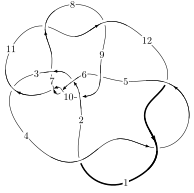
\includegraphics[width=112pt]{../../../GIT/diagram.site/Diagrams/png/1794_12a_0993.png}\\
\ \ \ A knot diagram\footnotemark}&
\allowdisplaybreaks
\textbf{Linearized knot diagam} \\
\cline{2-2}
 &
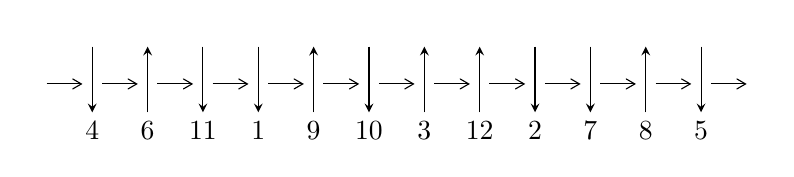
\begin{tikzpicture}[x=20pt, y=17pt]
	% nodes
	\node (C0) at (0, 0) {};
	\node (C1) at (1, 0) {};
	\node (C1U) at (1, +1) {};
	\node (C1D) at (1, -1) {4};

	\node (C2) at (2, 0) {};
	\node (C2U) at (2, +1) {};
	\node (C2D) at (2, -1) {6};

	\node (C3) at (3, 0) {};
	\node (C3U) at (3, +1) {};
	\node (C3D) at (3, -1) {11};

	\node (C4) at (4, 0) {};
	\node (C4U) at (4, +1) {};
	\node (C4D) at (4, -1) {1};

	\node (C5) at (5, 0) {};
	\node (C5U) at (5, +1) {};
	\node (C5D) at (5, -1) {9};

	\node (C6) at (6, 0) {};
	\node (C6U) at (6, +1) {};
	\node (C6D) at (6, -1) {10};

	\node (C7) at (7, 0) {};
	\node (C7U) at (7, +1) {};
	\node (C7D) at (7, -1) {3};

	\node (C8) at (8, 0) {};
	\node (C8U) at (8, +1) {};
	\node (C8D) at (8, -1) {12};

	\node (C9) at (9, 0) {};
	\node (C9U) at (9, +1) {};
	\node (C9D) at (9, -1) {2};

	\node (C10) at (10, 0) {};
	\node (C10U) at (10, +1) {};
	\node (C10D) at (10, -1) {7};

	\node (C11) at (11, 0) {};
	\node (C11U) at (11, +1) {};
	\node (C11D) at (11, -1) {8};

	\node (C12) at (12, 0) {};
	\node (C12U) at (12, +1) {};
	\node (C12D) at (12, -1) {5};
	\node (C13) at (13, 0) {};

	% arrows
	\draw[->,>={angle 60}]
	(C0) edge (C1) (C1) edge (C2) (C2) edge (C3) (C3) edge (C4) (C4) edge (C5) (C5) edge (C6) (C6) edge (C7) (C7) edge (C8) (C8) edge (C9) (C9) edge (C10) (C10) edge (C11) (C11) edge (C12) (C12) edge (C13) ;	\draw[->,>=stealth]
	(C1U) edge (C1D) (C2D) edge (C2U) (C3U) edge (C3D) (C4U) edge (C4D) (C5D) edge (C5U) (C6U) edge (C6D) (C7D) edge (C7U) (C8D) edge (C8U) (C9U) edge (C9D) (C10U) edge (C10D) (C11D) edge (C11U) (C12U) edge (C12D) ;
	\end{tikzpicture} \\
\hhline{~~} \\& 
\textbf{Solving Sequence} \\ \cline{2-2} 
 &
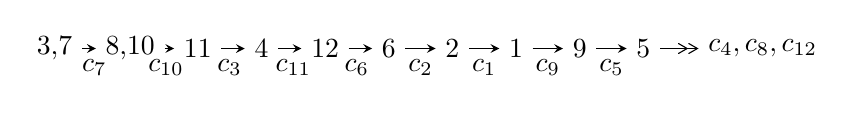
\begin{tikzpicture}[x=23pt, y=7pt]
	% node
	\node (A0) at (-1/8, 0) {3,7};
	\node (A1) at (17/16, 0) {8,10};
	\node (A2) at (17/8, 0) {11};
	\node (A3) at (25/8, 0) {4};
	\node (A4) at (33/8, 0) {12};
	\node (A5) at (41/8, 0) {6};
	\node (A6) at (49/8, 0) {2};
	\node (A7) at (57/8, 0) {1};
	\node (A8) at (65/8, 0) {9};
	\node (A9) at (73/8, 0) {5};
	\node (C1) at (1/2, -1) {$c_{7}$};
	\node (C2) at (13/8, -1) {$c_{10}$};
	\node (C3) at (21/8, -1) {$c_{3}$};
	\node (C4) at (29/8, -1) {$c_{11}$};
	\node (C5) at (37/8, -1) {$c_{6}$};
	\node (C6) at (45/8, -1) {$c_{2}$};
	\node (C7) at (53/8, -1) {$c_{1}$};
	\node (C8) at (61/8, -1) {$c_{9}$};
	\node (C9) at (69/8, -1) {$c_{5}$};
	\node (A10) at (11, 0) {$c_{4},c_{8},c_{12}$};

	% edge
	\draw[->,>=stealth]	
	(A0) edge (A1) (A1) edge (A2) (A2) edge (A3) (A3) edge (A4) (A4) edge (A5) (A5) edge (A6) (A6) edge (A7) (A7) edge (A8) (A8) edge (A9) ;
	\draw[->>,>={angle 60}]	
	(A9) edge (A10);
\end{tikzpicture} \\ 

\end{tabular} \\

\footnotetext{
The image of knot diagram is generated by the software ``\textbf{Draw programme}" developed by Andrew Bartholomew(\url{http://www.layer8.co.uk/maths/draw/index.htm\#Running-draw}), where we modified some parts for our purpose(\url{https://github.com/CATsTAILs/LinksPainter}).
}\phantom \\ \newline 
\centering \textbf{Ideals for irreducible components\footnotemark of $X_{\text{par}}$} 
 
\begin{align*}
I^u_{1}&=\langle 
1.10594\times10^{879} u^{125}+1.36630\times10^{879} u^{124}+\cdots+1.54517\times10^{880} b-3.26555\times10^{880},\\
\phantom{I^u_{1}}&\phantom{= \langle  }-8.92339\times10^{880} u^{125}-8.84509\times10^{880} u^{124}+\cdots+1.69969\times10^{881} a-7.52252\times10^{882},\\
\phantom{I^u_{1}}&\phantom{= \langle  }u^{126}+u^{125}+\cdots-132 u+11\rangle \\
I^u_{2}&=\langle 
-9.30719\times10^{30} u^{29}-5.87135\times10^{30} u^{28}+\cdots+1.66371\times10^{31} b+2.43132\times10^{31},\\
\phantom{I^u_{2}}&\phantom{= \langle  }-6.80425\times10^{30} u^{29}-4.64175\times10^{28} u^{28}+\cdots+1.66371\times10^{31} a-1.17316\times10^{31},\;u^{30}+3 u^{28}+\cdots-2 u-1\rangle \\
\\
\end{align*}
\raggedright * 2 irreducible components of $\dim_{\mathbb{C}}=0$, with total 156 representations.\\
\footnotetext{All coefficients of polynomials are rational numbers. But the coefficients are sometimes approximated in decimal forms when there is not enough margin.}
\newpage
\renewcommand{\arraystretch}{1}
\centering \section*{I. $I^u_{1}= \langle 1.11\times10^{879} u^{125}+1.37\times10^{879} u^{124}+\cdots+1.55\times10^{880} b-3.27\times10^{880},\;-8.92\times10^{880} u^{125}-8.85\times10^{880} u^{124}+\cdots+1.70\times10^{881} a-7.52\times10^{882},\;u^{126}+u^{125}+\cdots-132 u+11 \rangle$}
\flushleft \textbf{(i) Arc colorings}\\
\begin{tabular}{m{7pt} m{180pt} m{7pt} m{180pt} }
\flushright $a_{3}=$&$\begin{pmatrix}0\\u\end{pmatrix}$ \\
\flushright $a_{7}=$&$\begin{pmatrix}1\\0\end{pmatrix}$ \\
\flushright $a_{8}=$&$\begin{pmatrix}1\\- u^2\end{pmatrix}$ \\
\flushright $a_{10}=$&$\begin{pmatrix}0.525002 u^{125}+0.520395 u^{124}+\cdots-374.540 u+44.2583\\-0.0715738 u^{125}-0.0884238 u^{124}+\cdots-0.736350 u+2.11339\end{pmatrix}$ \\
\flushright $a_{11}=$&$\begin{pmatrix}0.596576 u^{125}+0.608819 u^{124}+\cdots-373.804 u+42.1449\\-0.0715738 u^{125}-0.0884238 u^{124}+\cdots-0.736350 u+2.11339\end{pmatrix}$ \\
\flushright $a_{4}=$&$\begin{pmatrix}1.58980 u^{125}+1.63087 u^{124}+\cdots-654.607 u-8.00754\\0.0966687 u^{125}+0.0928713 u^{124}+\cdots-91.2100 u+3.34168\end{pmatrix}$ \\
\flushright $a_{12}=$&$\begin{pmatrix}0.583221 u^{125}+0.593184 u^{124}+\cdots-379.487 u+44.1236\\-0.0729892 u^{125}-0.0918397 u^{124}+\cdots-0.582326 u+2.08831\end{pmatrix}$ \\
\flushright $a_{6}=$&$\begin{pmatrix}-0.259868 u^{125}-0.170339 u^{124}+\cdots+375.077 u-51.5973\\0.0439211 u^{125}+0.0367812 u^{124}+\cdots-27.1830 u-0.487529\end{pmatrix}$ \\
\flushright $a_{2}=$&$\begin{pmatrix}1.54565 u^{125}+1.31340 u^{124}+\cdots-1183.86 u+3.71872\\0.0592009 u^{125}+0.0546213 u^{124}+\cdots-46.3274 u-1.23676\end{pmatrix}$ \\
\flushright $a_{1}=$&$\begin{pmatrix}0.581766 u^{125}+0.450854 u^{124}+\cdots-139.927 u-31.3043\\-0.132150 u^{125}-0.220674 u^{124}+\cdots-81.3185 u+4.14573\end{pmatrix}$ \\
\flushright $a_{9}=$&$\begin{pmatrix}-0.180228 u^{125}+0.0908883 u^{124}+\cdots+625.815 u-72.6402\\0.0188578 u^{125}+0.0128273 u^{124}+\cdots-16.0604 u-1.06033\end{pmatrix}$ \\
\flushright $a_{5}=$&$\begin{pmatrix}-0.228010 u^{125}-0.696063 u^{124}+\cdots-619.877 u+37.7195\\0.0341963 u^{125}-0.0132225 u^{124}+\cdots-75.4933 u+3.53262\end{pmatrix}$\\&\end{tabular}
\flushleft \textbf{(ii) Obstruction class $= -1$}\\~\\
\flushleft \textbf{(iii) Cusp Shapes $= -0.0314101 u^{125}+0.232150 u^{124}+\cdots+485.494 u-43.2059$}\\~\\
\newpage\renewcommand{\arraystretch}{1}
\flushleft \textbf{(iv) u-Polynomials at the component}\newline \\
\begin{tabular}{m{50pt}|m{274pt}}
Crossings & \hspace{64pt}u-Polynomials at each crossing \\
\hline $$\begin{aligned}c_{1},c_{4},c_{12}\end{aligned}$$&$\begin{aligned}
&u^{126}+6 u^{125}+\cdots-46 u+1
\end{aligned}$\\
\hline $$\begin{aligned}c_{2}\end{aligned}$$&$\begin{aligned}
&u^{126}+6 u^{124}+\cdots+153 u-1
\end{aligned}$\\
\hline $$\begin{aligned}c_{3}\end{aligned}$$&$\begin{aligned}
&u^{126}+4 u^{124}+\cdots+13 u-1
\end{aligned}$\\
\hline $$\begin{aligned}c_{5}\end{aligned}$$&$\begin{aligned}
&u^{126}-7 u^{125}+\cdots+594874511 u-184550927
\end{aligned}$\\
\hline $$\begin{aligned}c_{6},c_{10}\end{aligned}$$&$\begin{aligned}
&u^{126}+u^{125}+\cdots-53 u-1
\end{aligned}$\\
\hline $$\begin{aligned}c_{7}\end{aligned}$$&$\begin{aligned}
&u^{126}+u^{125}+\cdots-132 u+11
\end{aligned}$\\
\hline $$\begin{aligned}c_{8},c_{11}\end{aligned}$$&$\begin{aligned}
&u^{126}-3 u^{125}+\cdots+64815 u-21157
\end{aligned}$\\
\hline $$\begin{aligned}c_{9}\end{aligned}$$&$\begin{aligned}
&u^{126}-3 u^{125}+\cdots-15150 u-875
\end{aligned}$\\
\hline
\end{tabular}\\~\\
\newpage\renewcommand{\arraystretch}{1}
\flushleft \textbf{(v) Riley Polynomials at the component}\newline \\
\begin{tabular}{m{50pt}|m{274pt}}
Crossings & \hspace{64pt}Riley Polynomials at each crossing \\
\hline $$\begin{aligned}c_{1},c_{4},c_{12}\end{aligned}$$&$\begin{aligned}
&y^{126}+128 y^{125}+\cdots-658 y+1
\end{aligned}$\\
\hline $$\begin{aligned}c_{2}\end{aligned}$$&$\begin{aligned}
&y^{126}+12 y^{125}+\cdots-25937 y+1
\end{aligned}$\\
\hline $$\begin{aligned}c_{3}\end{aligned}$$&$\begin{aligned}
&y^{126}+8 y^{125}+\cdots-539 y+1
\end{aligned}$\\
\hline $$\begin{aligned}c_{5}\end{aligned}$$&$\begin{aligned}
&y^{126}-61 y^{125}+\cdots-817860618458859723 y+34059044656559329
\end{aligned}$\\
\hline $$\begin{aligned}c_{6},c_{10}\end{aligned}$$&$\begin{aligned}
&y^{126}-89 y^{125}+\cdots-285 y+1
\end{aligned}$\\
\hline $$\begin{aligned}c_{7}\end{aligned}$$&$\begin{aligned}
&y^{126}- y^{125}+\cdots-28336 y+121
\end{aligned}$\\
\hline $$\begin{aligned}c_{8},c_{11}\end{aligned}$$&$\begin{aligned}
&y^{126}-107 y^{125}+\cdots+8032458629 y+447618649
\end{aligned}$\\
\hline $$\begin{aligned}c_{9}\end{aligned}$$&$\begin{aligned}
&y^{126}-13 y^{125}+\cdots-211112500 y+765625
\end{aligned}$\\
\hline
\end{tabular}\\~\\
\newpage\flushleft \textbf{(vi) Complex Volumes and Cusp Shapes}
$$\begin{array}{c|c|c}  
\text{Solutions to }I^u_{1}& \I (\text{vol} + \sqrt{-1}CS) & \text{Cusp shape}\\
 \hline 
\begin{aligned}
u &= \phantom{-}0.968012 + 0.206740 I \\
a &= -0.841309 + 0.618895 I \\
b &= \phantom{-}0.382176 - 0.612476 I\end{aligned}
 & \phantom{-}3.86360 - 1.13254 I & \phantom{-0.000000 } 0 \\ \hline\begin{aligned}
u &= \phantom{-}0.968012 - 0.206740 I \\
a &= -0.841309 - 0.618895 I \\
b &= \phantom{-}0.382176 + 0.612476 I\end{aligned}
 & \phantom{-}3.86360 + 1.13254 I & \phantom{-0.000000 } 0 \\ \hline\begin{aligned}
u &= \phantom{-}0.722580 + 0.707302 I \\
a &= \phantom{-}0.321355 - 0.392167 I \\
b &= \phantom{-}0.246993 - 0.037301 I\end{aligned}
 & \phantom{-}0.90720 + 2.23366 I & \phantom{-0.000000 } 0 \\ \hline\begin{aligned}
u &= \phantom{-}0.722580 - 0.707302 I \\
a &= \phantom{-}0.321355 + 0.392167 I \\
b &= \phantom{-}0.246993 + 0.037301 I\end{aligned}
 & \phantom{-}0.90720 - 2.23366 I & \phantom{-0.000000 } 0 \\ \hline\begin{aligned}
u &= -0.701722 + 0.731285 I \\
a &= \phantom{-}1.183870 - 0.557138 I \\
b &= \phantom{-}1.42066 + 0.47320 I\end{aligned}
 & -4.51319 - 2.95889 I & \phantom{-0.000000 } 0 \\ \hline\begin{aligned}
u &= -0.701722 - 0.731285 I \\
a &= \phantom{-}1.183870 + 0.557138 I \\
b &= \phantom{-}1.42066 - 0.47320 I\end{aligned}
 & -4.51319 + 2.95889 I & \phantom{-0.000000 } 0 \\ \hline\begin{aligned}
u &= -0.917887 + 0.351540 I \\
a &= \phantom{-}0.468009 - 0.083088 I \\
b &= -0.450872 + 0.696654 I\end{aligned}
 & \phantom{-}7.04474 - 1.32151 I & \phantom{-0.000000 } 0 \\ \hline\begin{aligned}
u &= -0.917887 - 0.351540 I \\
a &= \phantom{-}0.468009 + 0.083088 I \\
b &= -0.450872 - 0.696654 I\end{aligned}
 & \phantom{-}7.04474 + 1.32151 I & \phantom{-0.000000 } 0 \\ \hline\begin{aligned}
u &= -0.954461 + 0.202606 I \\
a &= -0.784825 - 1.021690 I \\
b &= \phantom{-}0.705378 + 0.641418 I\end{aligned}
 & \phantom{-}10.01000 + 3.91751 I & \phantom{-0.000000 } 0 \\ \hline\begin{aligned}
u &= -0.954461 - 0.202606 I \\
a &= -0.784825 + 1.021690 I \\
b &= \phantom{-}0.705378 - 0.641418 I\end{aligned}
 & \phantom{-}10.01000 - 3.91751 I & \phantom{-0.000000 } 0\\
 \hline 
 \end{array}$$\newpage$$\begin{array}{c|c|c}  
\text{Solutions to }I^u_{1}& \I (\text{vol} + \sqrt{-1}CS) & \text{Cusp shape}\\
 \hline 
\begin{aligned}
u &= \phantom{-}0.849912 + 0.583986 I \\
a &= -0.373182 - 1.071840 I \\
b &= -1.163970 + 0.238978 I\end{aligned}
 & \phantom{-}0.47499 + 5.28536 I & \phantom{-0.000000 } 0 \\ \hline\begin{aligned}
u &= \phantom{-}0.849912 - 0.583986 I \\
a &= -0.373182 + 1.071840 I \\
b &= -1.163970 - 0.238978 I\end{aligned}
 & \phantom{-}0.47499 - 5.28536 I & \phantom{-0.000000 } 0 \\ \hline\begin{aligned}
u &= -0.737965 + 0.626114 I \\
a &= \phantom{-}0.510029 - 0.263258 I \\
b &= -0.157910 + 1.032840 I\end{aligned}
 & \phantom{-}6.41264 - 2.33812 I & \phantom{-0.000000 } 0 \\ \hline\begin{aligned}
u &= -0.737965 - 0.626114 I \\
a &= \phantom{-}0.510029 + 0.263258 I \\
b &= -0.157910 - 1.032840 I\end{aligned}
 & \phantom{-}6.41264 + 2.33812 I & \phantom{-0.000000 } 0 \\ \hline\begin{aligned}
u &= -0.129149 + 0.954019 I \\
a &= \phantom{-}1.237170 + 0.019775 I \\
b &= \phantom{-}1.30144 + 0.76450 I\end{aligned}
 & \phantom{-}3.05595 - 3.53054 I & \phantom{-0.000000 } 0 \\ \hline\begin{aligned}
u &= -0.129149 - 0.954019 I \\
a &= \phantom{-}1.237170 - 0.019775 I \\
b &= \phantom{-}1.30144 - 0.76450 I\end{aligned}
 & \phantom{-}3.05595 + 3.53054 I & \phantom{-0.000000 } 0 \\ \hline\begin{aligned}
u &= -0.269534 + 0.918113 I \\
a &= \phantom{-}1.052230 - 0.391170 I \\
b &= \phantom{-}0.573678 + 0.616502 I\end{aligned}
 & \phantom{-}4.73137 - 2.68223 I & \phantom{-0.000000 } 0 \\ \hline\begin{aligned}
u &= -0.269534 - 0.918113 I \\
a &= \phantom{-}1.052230 + 0.391170 I \\
b &= \phantom{-}0.573678 - 0.616502 I\end{aligned}
 & \phantom{-}4.73137 + 2.68223 I & \phantom{-0.000000 } 0 \\ \hline\begin{aligned}
u &= -0.037847 + 1.063370 I \\
a &= -1.076550 + 0.583214 I \\
b &= \phantom{-}0.0644537 + 0.1137520 I\end{aligned}
 & \phantom{-}9.63649 - 7.24665 I & \phantom{-0.000000 } 0 \\ \hline\begin{aligned}
u &= -0.037847 - 1.063370 I \\
a &= -1.076550 - 0.583214 I \\
b &= \phantom{-}0.0644537 - 0.1137520 I\end{aligned}
 & \phantom{-}9.63649 + 7.24665 I & \phantom{-0.000000 } 0\\
 \hline 
 \end{array}$$\newpage$$\begin{array}{c|c|c}  
\text{Solutions to }I^u_{1}& \I (\text{vol} + \sqrt{-1}CS) & \text{Cusp shape}\\
 \hline 
\begin{aligned}
u &= \phantom{-}0.779491 + 0.757708 I \\
a &= \phantom{-}1.02597 + 2.06833 I \\
b &= \phantom{-}1.154720 - 0.147525 I\end{aligned}
 & \phantom{-}6.63909 + 8.20125 I & \phantom{-0.000000 } 0 \\ \hline\begin{aligned}
u &= \phantom{-}0.779491 - 0.757708 I \\
a &= \phantom{-}1.02597 - 2.06833 I \\
b &= \phantom{-}1.154720 + 0.147525 I\end{aligned}
 & \phantom{-}6.63909 - 8.20125 I & \phantom{-0.000000 } 0 \\ \hline\begin{aligned}
u &= \phantom{-}0.174729 + 0.889388 I \\
a &= \phantom{-}1.44002 - 0.73130 I \\
b &= \phantom{-}0.440431 + 0.046106 I\end{aligned}
 & \phantom{-}4.69795 - 2.86828 I & \phantom{-0.000000 } 0 \\ \hline\begin{aligned}
u &= \phantom{-}0.174729 - 0.889388 I \\
a &= \phantom{-}1.44002 + 0.73130 I \\
b &= \phantom{-}0.440431 - 0.046106 I\end{aligned}
 & \phantom{-}4.69795 + 2.86828 I & \phantom{-0.000000 } 0 \\ \hline\begin{aligned}
u &= \phantom{-}0.026878 + 0.904424 I \\
a &= -2.23187 - 0.74246 I \\
b &= -1.161310 - 0.131568 I\end{aligned}
 & -2.91584 - 3.59853 I & \phantom{-0.000000 } 0 \\ \hline\begin{aligned}
u &= \phantom{-}0.026878 - 0.904424 I \\
a &= -2.23187 + 0.74246 I \\
b &= -1.161310 + 0.131568 I\end{aligned}
 & -2.91584 + 3.59853 I & \phantom{-0.000000 } 0 \\ \hline\begin{aligned}
u &= \phantom{-}0.738162 + 0.516805 I \\
a &= \phantom{-}1.112750 + 0.775174 I \\
b &= \phantom{-}1.43589 - 0.61909 I\end{aligned}
 & -0.64593 + 6.02874 I & \phantom{-0.000000 } 0 \\ \hline\begin{aligned}
u &= \phantom{-}0.738162 - 0.516805 I \\
a &= \phantom{-}1.112750 - 0.775174 I \\
b &= \phantom{-}1.43589 + 0.61909 I\end{aligned}
 & -0.64593 - 6.02874 I & \phantom{-0.000000 } 0 \\ \hline\begin{aligned}
u &= -1.036500 + 0.425597 I \\
a &= -0.643009 - 0.175995 I \\
b &= -0.174290 + 0.707571 I\end{aligned}
 & \phantom{-}4.76622 - 2.24293 I & \phantom{-0.000000 } 0 \\ \hline\begin{aligned}
u &= -1.036500 - 0.425597 I \\
a &= -0.643009 + 0.175995 I \\
b &= -0.174290 - 0.707571 I\end{aligned}
 & \phantom{-}4.76622 + 2.24293 I & \phantom{-0.000000 } 0\\
 \hline 
 \end{array}$$\newpage$$\begin{array}{c|c|c}  
\text{Solutions to }I^u_{1}& \I (\text{vol} + \sqrt{-1}CS) & \text{Cusp shape}\\
 \hline 
\begin{aligned}
u &= -0.399858 + 1.062710 I \\
a &= \phantom{-}2.54526 - 1.21520 I \\
b &= \phantom{-}1.150700 + 0.055423 I\end{aligned}
 & -0.70367 - 3.42936 I & \phantom{-0.000000 } 0 \\ \hline\begin{aligned}
u &= -0.399858 - 1.062710 I \\
a &= \phantom{-}2.54526 + 1.21520 I \\
b &= \phantom{-}1.150700 - 0.055423 I\end{aligned}
 & -0.70367 + 3.42936 I & \phantom{-0.000000 } 0 \\ \hline\begin{aligned}
u &= -0.501362 + 0.698749 I \\
a &= -1.10159 + 1.68091 I \\
b &= -1.160730 - 0.040659 I\end{aligned}
 & -4.55735 - 1.27291 I & \phantom{-0.000000 } 0 \\ \hline\begin{aligned}
u &= -0.501362 - 0.698749 I \\
a &= -1.10159 - 1.68091 I \\
b &= -1.160730 + 0.040659 I\end{aligned}
 & -4.55735 + 1.27291 I & \phantom{-0.000000 } 0 \\ \hline\begin{aligned}
u &= \phantom{-}0.767040 + 0.378405 I \\
a &= -1.367770 + 0.112888 I \\
b &= -1.59069 - 0.13500 I\end{aligned}
 & \phantom{-}7.20930 - 3.74478 I & \phantom{-0.000000 } 0 \\ \hline\begin{aligned}
u &= \phantom{-}0.767040 - 0.378405 I \\
a &= -1.367770 - 0.112888 I \\
b &= -1.59069 + 0.13500 I\end{aligned}
 & \phantom{-}7.20930 + 3.74478 I & \phantom{-0.000000 } 0 \\ \hline\begin{aligned}
u &= \phantom{-}0.662164 + 0.494308 I \\
a &= \phantom{-}0.334236 + 0.339193 I \\
b &= -0.150099 - 0.914798 I\end{aligned}
 & \phantom{-}1.19579 + 1.85580 I & \phantom{-0.000000 } 0 \\ \hline\begin{aligned}
u &= \phantom{-}0.662164 - 0.494308 I \\
a &= \phantom{-}0.334236 - 0.339193 I \\
b &= -0.150099 + 0.914798 I\end{aligned}
 & \phantom{-}1.19579 - 1.85580 I & \phantom{-0.000000 } 0 \\ \hline\begin{aligned}
u &= \phantom{-}0.751275 + 0.914799 I \\
a &= \phantom{-}1.110060 + 0.454273 I \\
b &= \phantom{-}1.45340 - 0.27676 I\end{aligned}
 & -0.695593 + 0.430873 I & \phantom{-0.000000 } 0 \\ \hline\begin{aligned}
u &= \phantom{-}0.751275 - 0.914799 I \\
a &= \phantom{-}1.110060 - 0.454273 I \\
b &= \phantom{-}1.45340 + 0.27676 I\end{aligned}
 & -0.695593 - 0.430873 I & \phantom{-0.000000 } 0\\
 \hline 
 \end{array}$$\newpage$$\begin{array}{c|c|c}  
\text{Solutions to }I^u_{1}& \I (\text{vol} + \sqrt{-1}CS) & \text{Cusp shape}\\
 \hline 
\begin{aligned}
u &= \phantom{-}0.539342 + 0.609694 I \\
a &= -2.44519 - 1.07402 I \\
b &= -1.046790 + 0.382026 I\end{aligned}
 & \phantom{-}5.19982 + 5.44798 I & \phantom{-0.000000 } 0. - 8.13519 I \\ \hline\begin{aligned}
u &= \phantom{-}0.539342 - 0.609694 I \\
a &= -2.44519 + 1.07402 I \\
b &= -1.046790 - 0.382026 I\end{aligned}
 & \phantom{-}5.19982 - 5.44798 I & \phantom{-0.000000 -}0. + 8.13519 I \\ \hline\begin{aligned}
u &= \phantom{-}0.727479 + 0.334456 I \\
a &= \phantom{-}0.336265 - 0.041580 I \\
b &= -0.036714 - 0.666665 I\end{aligned}
 & \phantom{-}1.04572 + 1.34644 I & \phantom{-0.000000 } 0 \\ \hline\begin{aligned}
u &= \phantom{-}0.727479 - 0.334456 I \\
a &= \phantom{-}0.336265 + 0.041580 I \\
b &= -0.036714 + 0.666665 I\end{aligned}
 & \phantom{-}1.04572 - 1.34644 I & \phantom{-0.000000 } 0 \\ \hline\begin{aligned}
u &= \phantom{-}0.136225 + 0.776984 I \\
a &= \phantom{-}1.46727 - 0.01362 I \\
b &= \phantom{-}1.31564 - 0.63453 I\end{aligned}
 & -2.11477 + 2.94281 I & -23.2919 - 10.5595 I \\ \hline\begin{aligned}
u &= \phantom{-}0.136225 - 0.776984 I \\
a &= \phantom{-}1.46727 + 0.01362 I \\
b &= \phantom{-}1.31564 + 0.63453 I\end{aligned}
 & -2.11477 - 2.94281 I & -23.2919 + 10.5595 I \\ \hline\begin{aligned}
u &= -0.788165\phantom{ +0.000000I} \\
a &= -1.55663\phantom{ +0.000000I} \\
b &= -1.39953\phantom{ +0.000000I}\end{aligned}
 & \phantom{-}2.48354\phantom{ +0.000000I} & \phantom{-}5.67410\phantom{ +0.000000I} \\ \hline\begin{aligned}
u &= \phantom{-}0.090736 + 1.219680 I \\
a &= -0.686362 - 0.249825 I \\
b &= \phantom{-}0.0687145 - 0.0314972 I\end{aligned}
 & \phantom{-}2.19489 + 3.04393 I & \phantom{-0.000000 } 0 \\ \hline\begin{aligned}
u &= \phantom{-}0.090736 - 1.219680 I \\
a &= -0.686362 + 0.249825 I \\
b &= \phantom{-}0.0687145 + 0.0314972 I\end{aligned}
 & \phantom{-}2.19489 - 3.04393 I & \phantom{-0.000000 } 0 \\ \hline\begin{aligned}
u &= \phantom{-}1.026350 + 0.680770 I \\
a &= -0.0526145 + 0.0042219 I \\
b &= -0.078455 + 1.177730 I\end{aligned}
 & \phantom{-}12.1495 + 12.5348 I & \phantom{-0.000000 } 0\\
 \hline 
 \end{array}$$\newpage$$\begin{array}{c|c|c}  
\text{Solutions to }I^u_{1}& \I (\text{vol} + \sqrt{-1}CS) & \text{Cusp shape}\\
 \hline 
\begin{aligned}
u &= \phantom{-}1.026350 - 0.680770 I \\
a &= -0.0526145 - 0.0042219 I \\
b &= -0.078455 - 1.177730 I\end{aligned}
 & \phantom{-}12.1495 - 12.5348 I & \phantom{-0.000000 } 0 \\ \hline\begin{aligned}
u &= -1.073650 + 0.642604 I \\
a &= -0.0280392 + 0.0269565 I \\
b &= -0.136979 - 1.044980 I\end{aligned}
 & \phantom{-}5.48825 - 8.57859 I & \phantom{-0.000000 } 0 \\ \hline\begin{aligned}
u &= -1.073650 - 0.642604 I \\
a &= -0.0280392 - 0.0269565 I \\
b &= -0.136979 + 1.044980 I\end{aligned}
 & \phantom{-}5.48825 + 8.57859 I & \phantom{-0.000000 } 0 \\ \hline\begin{aligned}
u &= \phantom{-}0.428583 + 1.180290 I \\
a &= \phantom{-}1.189860 + 0.294886 I \\
b &= \phantom{-}1.009070 - 0.273860 I\end{aligned}
 & -1.42765 + 1.64320 I & \phantom{-0.000000 } 0 \\ \hline\begin{aligned}
u &= \phantom{-}0.428583 - 1.180290 I \\
a &= \phantom{-}1.189860 - 0.294886 I \\
b &= \phantom{-}1.009070 + 0.273860 I\end{aligned}
 & -1.42765 - 1.64320 I & \phantom{-0.000000 } 0 \\ \hline\begin{aligned}
u &= -0.693722 + 0.261825 I \\
a &= -0.264784 - 0.486947 I \\
b &= -0.211354 + 1.166350 I\end{aligned}
 & \phantom{-}4.43559 - 0.75434 I & \phantom{-}7.78662 - 2.19445 I \\ \hline\begin{aligned}
u &= -0.693722 - 0.261825 I \\
a &= -0.264784 + 0.486947 I \\
b &= -0.211354 - 1.166350 I\end{aligned}
 & \phantom{-}4.43559 + 0.75434 I & \phantom{-}7.78662 + 2.19445 I \\ \hline\begin{aligned}
u &= \phantom{-}1.070930 + 0.704608 I \\
a &= -0.618275 - 0.024661 I \\
b &= -0.509253 - 0.785700 I\end{aligned}
 & \phantom{-}11.83960 + 4.23093 I & \phantom{-0.000000 } 0 \\ \hline\begin{aligned}
u &= \phantom{-}1.070930 - 0.704608 I \\
a &= -0.618275 + 0.024661 I \\
b &= -0.509253 + 0.785700 I\end{aligned}
 & \phantom{-}11.83960 - 4.23093 I & \phantom{-0.000000 } 0 \\ \hline\begin{aligned}
u &= \phantom{-}0.511429 + 0.500117 I \\
a &= -0.217174 - 0.188538 I \\
b &= \phantom{-}0.026842 - 1.328720 I\end{aligned}
 & \phantom{-}5.71723 + 5.77036 I & \phantom{-}2.36112 - 11.11424 I\\
 \hline 
 \end{array}$$\newpage$$\begin{array}{c|c|c}  
\text{Solutions to }I^u_{1}& \I (\text{vol} + \sqrt{-1}CS) & \text{Cusp shape}\\
 \hline 
\begin{aligned}
u &= \phantom{-}0.511429 - 0.500117 I \\
a &= -0.217174 + 0.188538 I \\
b &= \phantom{-}0.026842 + 1.328720 I\end{aligned}
 & \phantom{-}5.71723 - 5.77036 I & \phantom{-}2.36112 + 11.11424 I \\ \hline\begin{aligned}
u &= -0.749688 + 1.044300 I \\
a &= -1.55802 + 0.39336 I \\
b &= -1.326070 - 0.393163 I\end{aligned}
 & -3.18376 - 5.37366 I & \phantom{-0.000000 } 0 \\ \hline\begin{aligned}
u &= -0.749688 - 1.044300 I \\
a &= -1.55802 - 0.39336 I \\
b &= -1.326070 + 0.393163 I\end{aligned}
 & -3.18376 + 5.37366 I & \phantom{-0.000000 } 0 \\ \hline\begin{aligned}
u &= \phantom{-}1.030840 + 0.770617 I \\
a &= -1.11660 - 1.00027 I \\
b &= -1.32126 + 0.58253 I\end{aligned}
 & \phantom{-}2.78831 + 8.21347 I & \phantom{-0.000000 } 0 \\ \hline\begin{aligned}
u &= \phantom{-}1.030840 - 0.770617 I \\
a &= -1.11660 + 1.00027 I \\
b &= -1.32126 - 0.58253 I\end{aligned}
 & \phantom{-}2.78831 - 8.21347 I & \phantom{-0.000000 } 0 \\ \hline\begin{aligned}
u &= \phantom{-}1.30548\phantom{ +0.000000I} \\
a &= \phantom{-}0.413226\phantom{ +0.000000I} \\
b &= -0.995775\phantom{ +0.000000I}\end{aligned}
 & \phantom{-}3.28667\phantom{ +0.000000I} & \phantom{-0.000000 } 0 \\ \hline\begin{aligned}
u &= -1.311650 + 0.039307 I \\
a &= \phantom{-}0.428074 - 0.025182 I \\
b &= -1.040940 + 0.127080 I\end{aligned}
 & \phantom{-}8.28404 - 0.19696 I & \phantom{-0.000000 } 0 \\ \hline\begin{aligned}
u &= -1.311650 - 0.039307 I \\
a &= \phantom{-}0.428074 + 0.025182 I \\
b &= -1.040940 - 0.127080 I\end{aligned}
 & \phantom{-}8.28404 + 0.19696 I & \phantom{-0.000000 } 0 \\ \hline\begin{aligned}
u &= -0.568653 + 0.381095 I \\
a &= -0.041833 + 0.196380 I \\
b &= \phantom{-}0.175657 + 1.110410 I\end{aligned}
 & \phantom{-}0.21103 - 3.56176 I & -2.00000 + 12.87689 I \\ \hline\begin{aligned}
u &= -0.568653 - 0.381095 I \\
a &= -0.041833 - 0.196380 I \\
b &= \phantom{-}0.175657 - 1.110410 I\end{aligned}
 & \phantom{-}0.21103 + 3.56176 I & -2.00000 - 12.87689 I\\
 \hline 
 \end{array}$$\newpage$$\begin{array}{c|c|c}  
\text{Solutions to }I^u_{1}& \I (\text{vol} + \sqrt{-1}CS) & \text{Cusp shape}\\
 \hline 
\begin{aligned}
u &= -1.017290 + 0.849259 I \\
a &= -1.138810 + 0.819126 I \\
b &= -1.312060 - 0.520361 I\end{aligned}
 & -2.50148 - 7.21721 I & \phantom{-0.000000 } 0 \\ \hline\begin{aligned}
u &= -1.017290 - 0.849259 I \\
a &= -1.138810 - 0.819126 I \\
b &= -1.312060 + 0.520361 I\end{aligned}
 & -2.50148 + 7.21721 I & \phantom{-0.000000 } 0 \\ \hline\begin{aligned}
u &= \phantom{-}1.161240 + 0.645349 I \\
a &= \phantom{-}0.0269442 - 0.0391937 I \\
b &= -0.083701 + 0.838821 I\end{aligned}
 & \phantom{-}5.69849 + 3.36426 I & \phantom{-0.000000 } 0 \\ \hline\begin{aligned}
u &= \phantom{-}1.161240 - 0.645349 I \\
a &= \phantom{-}0.0269442 + 0.0391937 I \\
b &= -0.083701 - 0.838821 I\end{aligned}
 & \phantom{-}5.69849 - 3.36426 I & \phantom{-0.000000 } 0 \\ \hline\begin{aligned}
u &= -0.225504 + 0.603291 I \\
a &= \phantom{-}0.926505 + 0.688105 I \\
b &= \phantom{-}0.171819 - 0.041861 I\end{aligned}
 & -1.034390 + 0.819414 I & -7.05388 - 2.21568 I \\ \hline\begin{aligned}
u &= -0.225504 - 0.603291 I \\
a &= \phantom{-}0.926505 - 0.688105 I \\
b &= \phantom{-}0.171819 + 0.041861 I\end{aligned}
 & -1.034390 - 0.819414 I & -7.05388 + 2.21568 I \\ \hline\begin{aligned}
u &= -1.029170 + 0.904792 I \\
a &= \phantom{-}0.970558 - 0.328742 I \\
b &= \phantom{-}1.160940 - 0.071700 I\end{aligned}
 & -2.77637 + 0.66825 I & \phantom{-0.000000 } 0 \\ \hline\begin{aligned}
u &= -1.029170 - 0.904792 I \\
a &= \phantom{-}0.970558 + 0.328742 I \\
b &= \phantom{-}1.160940 + 0.071700 I\end{aligned}
 & -2.77637 - 0.66825 I & \phantom{-0.000000 } 0 \\ \hline\begin{aligned}
u &= \phantom{-}0.305187 + 0.546803 I \\
a &= \phantom{-}1.25848 + 0.71590 I \\
b &= \phantom{-}1.36172 + 0.53318 I\end{aligned}
 & \phantom{-}1.77844 - 2.71652 I & \phantom{-}0.434746 - 0.863996 I \\ \hline\begin{aligned}
u &= \phantom{-}0.305187 - 0.546803 I \\
a &= \phantom{-}1.25848 - 0.71590 I \\
b &= \phantom{-}1.36172 - 0.53318 I\end{aligned}
 & \phantom{-}1.77844 + 2.71652 I & \phantom{-}0.434746 + 0.863996 I\\
 \hline 
 \end{array}$$\newpage$$\begin{array}{c|c|c}  
\text{Solutions to }I^u_{1}& \I (\text{vol} + \sqrt{-1}CS) & \text{Cusp shape}\\
 \hline 
\begin{aligned}
u &= \phantom{-}0.861315 + 1.089700 I \\
a &= -1.341780 - 0.385251 I \\
b &= -1.38682 + 0.49565 I\end{aligned}
 & -4.57772 + 9.15194 I & \phantom{-0.000000 } 0 \\ \hline\begin{aligned}
u &= \phantom{-}0.861315 - 1.089700 I \\
a &= -1.341780 + 0.385251 I \\
b &= -1.38682 - 0.49565 I\end{aligned}
 & -4.57772 - 9.15194 I & \phantom{-0.000000 } 0 \\ \hline\begin{aligned}
u &= -1.199660 + 0.737164 I \\
a &= \phantom{-}0.0783001 - 0.0072274 I \\
b &= \phantom{-}0.175996 - 0.762885 I\end{aligned}
 & \phantom{-}12.86710 + 0.42464 I & \phantom{-0.000000 } 0 \\ \hline\begin{aligned}
u &= -1.199660 - 0.737164 I \\
a &= \phantom{-}0.0783001 + 0.0072274 I \\
b &= \phantom{-}0.175996 + 0.762885 I\end{aligned}
 & \phantom{-}12.86710 - 0.42464 I & \phantom{-0.000000 } 0 \\ \hline\begin{aligned}
u &= -0.89430 + 1.13406 I \\
a &= -1.261770 + 0.364178 I \\
b &= -1.39930 - 0.57543 I\end{aligned}
 & \phantom{-}1.23096 - 12.20610 I & \phantom{-0.000000 } 0 \\ \hline\begin{aligned}
u &= -0.89430 - 1.13406 I \\
a &= -1.261770 - 0.364178 I \\
b &= -1.39930 + 0.57543 I\end{aligned}
 & \phantom{-}1.23096 + 12.20610 I & \phantom{-0.000000 } 0 \\ \hline\begin{aligned}
u &= \phantom{-}0.453539 + 0.307718 I \\
a &= \phantom{-}0.837401 + 0.907158 I \\
b &= \phantom{-}1.233150 + 0.594856 I\end{aligned}
 & \phantom{-}1.78881 - 2.72875 I & \phantom{-}2.39765 + 0.46040 I \\ \hline\begin{aligned}
u &= \phantom{-}0.453539 - 0.307718 I \\
a &= \phantom{-}0.837401 - 0.907158 I \\
b &= \phantom{-}1.233150 - 0.594856 I\end{aligned}
 & \phantom{-}1.78881 + 2.72875 I & \phantom{-}2.39765 - 0.46040 I \\ \hline\begin{aligned}
u &= \phantom{-}1.15430 + 0.88730 I \\
a &= -0.924165 - 0.603908 I \\
b &= -1.293110 + 0.434196 I\end{aligned}
 & \phantom{-}0.75691 + 6.06319 I & \phantom{-0.000000 } 0 \\ \hline\begin{aligned}
u &= \phantom{-}1.15430 - 0.88730 I \\
a &= -0.924165 + 0.603908 I \\
b &= -1.293110 - 0.434196 I\end{aligned}
 & \phantom{-}0.75691 - 6.06319 I & \phantom{-0.000000 } 0\\
 \hline 
 \end{array}$$\newpage$$\begin{array}{c|c|c}  
\text{Solutions to }I^u_{1}& \I (\text{vol} + \sqrt{-1}CS) & \text{Cusp shape}\\
 \hline 
\begin{aligned}
u &= \phantom{-}0.480589 + 0.170637 I \\
a &= -0.972704 + 0.672663 I \\
b &= -1.126390 - 0.834072 I\end{aligned}
 & \phantom{-}2.45303 + 2.40939 I & \phantom{-}9.70516 - 8.98371 I \\ \hline\begin{aligned}
u &= \phantom{-}0.480589 - 0.170637 I \\
a &= -0.972704 - 0.672663 I \\
b &= -1.126390 + 0.834072 I\end{aligned}
 & \phantom{-}2.45303 - 2.40939 I & \phantom{-}9.70516 + 8.98371 I \\ \hline\begin{aligned}
u &= \phantom{-}0.478856 + 0.007166 I \\
a &= -3.70484 - 1.81326 I \\
b &= -0.717751 + 0.180802 I\end{aligned}
 & \phantom{-}9.23772 + 1.58715 I & \phantom{-}0.97417 - 3.87239 I \\ \hline\begin{aligned}
u &= \phantom{-}0.478856 - 0.007166 I \\
a &= -3.70484 + 1.81326 I \\
b &= -0.717751 - 0.180802 I\end{aligned}
 & \phantom{-}9.23772 - 1.58715 I & \phantom{-}0.97417 + 3.87239 I \\ \hline\begin{aligned}
u &= -0.466435 + 0.066221 I \\
a &= -2.15123 - 1.42660 I \\
b &= -0.859954 + 0.294542 I\end{aligned}
 & \phantom{-}2.90713 + 0.56914 I & \phantom{-}2.73109 - 0.87226 I \\ \hline\begin{aligned}
u &= -0.466435 - 0.066221 I \\
a &= -2.15123 + 1.42660 I \\
b &= -0.859954 - 0.294542 I\end{aligned}
 & \phantom{-}2.90713 - 0.56914 I & \phantom{-}2.73109 + 0.87226 I \\ \hline\begin{aligned}
u &= -0.427326 + 0.179054 I \\
a &= -0.948841 - 0.387226 I \\
b &= -1.49741 + 1.02920 I\end{aligned}
 & \phantom{-}8.21252 - 5.33315 I & \phantom{-}19.4828 + 13.2523 I \\ \hline\begin{aligned}
u &= -0.427326 - 0.179054 I \\
a &= -0.948841 + 0.387226 I \\
b &= -1.49741 - 1.02920 I\end{aligned}
 & \phantom{-}8.21252 + 5.33315 I & \phantom{-}19.4828 - 13.2523 I \\ \hline\begin{aligned}
u &= -1.25961 + 1.08912 I \\
a &= \phantom{-}1.263630 - 0.518184 I \\
b &= \phantom{-}1.39968 + 0.54420 I\end{aligned}
 & \phantom{-}7.5384 - 18.5486 I & \phantom{-0.000000 } 0 \\ \hline\begin{aligned}
u &= -1.25961 - 1.08912 I \\
a &= \phantom{-}1.263630 + 0.518184 I \\
b &= \phantom{-}1.39968 - 0.54420 I\end{aligned}
 & \phantom{-}7.5384 + 18.5486 I & \phantom{-0.000000 } 0\\
 \hline 
 \end{array}$$\newpage$$\begin{array}{c|c|c}  
\text{Solutions to }I^u_{1}& \I (\text{vol} + \sqrt{-1}CS) & \text{Cusp shape}\\
 \hline 
\begin{aligned}
u &= \phantom{-}1.13918 + 1.26493 I \\
a &= \phantom{-}1.43226 + 0.45253 I \\
b &= \phantom{-}1.175520 - 0.398048 I\end{aligned}
 & \phantom{-}9.79810 + 3.83465 I & \phantom{-0.000000 } 0 \\ \hline\begin{aligned}
u &= \phantom{-}1.13918 - 1.26493 I \\
a &= \phantom{-}1.43226 - 0.45253 I \\
b &= \phantom{-}1.175520 + 0.398048 I\end{aligned}
 & \phantom{-}9.79810 - 3.83465 I & \phantom{-0.000000 } 0 \\ \hline\begin{aligned}
u &= \phantom{-}0.254512 + 0.147816 I \\
a &= -1.96888 - 7.45158 I \\
b &= \phantom{-}0.882430 + 0.329821 I\end{aligned}
 & \phantom{-}9.53051 - 7.93705 I & \phantom{-}6.98604 + 6.82257 I \\ \hline\begin{aligned}
u &= \phantom{-}0.254512 - 0.147816 I \\
a &= -1.96888 + 7.45158 I \\
b &= \phantom{-}0.882430 - 0.329821 I\end{aligned}
 & \phantom{-}9.53051 + 7.93705 I & \phantom{-}6.98604 - 6.82257 I \\ \hline\begin{aligned}
u &= \phantom{-}1.29164 + 1.11912 I \\
a &= \phantom{-}1.281340 + 0.476994 I \\
b &= \phantom{-}1.38748 - 0.48196 I\end{aligned}
 & \phantom{-}0.73747 + 13.98510 I & \phantom{-0.000000 } 0 \\ \hline\begin{aligned}
u &= \phantom{-}1.29164 - 1.11912 I \\
a &= \phantom{-}1.281340 - 0.476994 I \\
b &= \phantom{-}1.38748 + 0.48196 I\end{aligned}
 & \phantom{-}0.73747 - 13.98510 I & \phantom{-0.000000 } 0 \\ \hline\begin{aligned}
u &= -1.29864 + 1.20884 I \\
a &= \phantom{-}1.333510 - 0.438800 I \\
b &= \phantom{-}1.330460 + 0.411568 I\end{aligned}
 & \phantom{-}1.29402 - 7.90745 I & \phantom{-0.000000 } 0 \\ \hline\begin{aligned}
u &= -1.29864 - 1.20884 I \\
a &= \phantom{-}1.333510 + 0.438800 I \\
b &= \phantom{-}1.330460 - 0.411568 I\end{aligned}
 & \phantom{-}1.29402 + 7.90745 I & \phantom{-0.000000 } 0 \\ \hline\begin{aligned}
u &= -0.193279 + 0.005870 I \\
a &= \phantom{-}5.89648 + 8.48690 I \\
b &= \phantom{-}1.090150 - 0.280523 I\end{aligned}
 & \phantom{-}1.73678 + 4.67643 I & \phantom{-}0.44528 - 8.40035 I \\ \hline\begin{aligned}
u &= -0.193279 - 0.005870 I \\
a &= \phantom{-}5.89648 - 8.48690 I \\
b &= \phantom{-}1.090150 + 0.280523 I\end{aligned}
 & \phantom{-}1.73678 - 4.67643 I & \phantom{-}0.44528 + 8.40035 I\\
 \hline 
 \end{array}$$\newpage$$\begin{array}{c|c|c}  
\text{Solutions to }I^u_{1}& \I (\text{vol} + \sqrt{-1}CS) & \text{Cusp shape}\\
 \hline 
\begin{aligned}
u &= -1.52049 + 0.98628 I \\
a &= \phantom{-}0.640257 - 0.378084 I \\
b &= \phantom{-}1.100000 - 0.152001 I\end{aligned}
 & \phantom{-}2.65701 + 4.12493 I & \phantom{-0.000000 } 0 \\ \hline\begin{aligned}
u &= -1.52049 - 0.98628 I \\
a &= \phantom{-}0.640257 + 0.378084 I \\
b &= \phantom{-}1.100000 + 0.152001 I\end{aligned}
 & \phantom{-}2.65701 - 4.12493 I & \phantom{-0.000000 } 0 \\ \hline\begin{aligned}
u &= -1.07511 + 1.47313 I \\
a &= \phantom{-}1.291260 - 0.469674 I \\
b &= \phantom{-}1.120550 + 0.097386 I\end{aligned}
 & -1.48943 - 3.08194 I & \phantom{-0.000000 } 0 \\ \hline\begin{aligned}
u &= -1.07511 - 1.47313 I \\
a &= \phantom{-}1.291260 + 0.469674 I \\
b &= \phantom{-}1.120550 - 0.097386 I\end{aligned}
 & -1.48943 + 3.08194 I & \phantom{-0.000000 } 0 \\ \hline\begin{aligned}
u &= \phantom{-}0.0850834\phantom{ +0.000000I} \\
a &= \phantom{-}19.3001\phantom{ +0.000000I} \\
b &= \phantom{-}1.28315\phantom{ +0.000000I}\end{aligned}
 & -0.636876\phantom{ +0.000000I} & -8.64910\phantom{ +0.000000I} \\ \hline\begin{aligned}
u &= -1.24844 + 1.45738 I \\
a &= -1.077590 + 0.267882 I \\
b &= -0.995158 - 0.410825 I\end{aligned}
 & \phantom{-}10.31510 - 8.71832 I & \phantom{-0.000000 } 0 \\ \hline\begin{aligned}
u &= -1.24844 - 1.45738 I \\
a &= -1.077590 - 0.267882 I \\
b &= -0.995158 + 0.410825 I\end{aligned}
 & \phantom{-}10.31510 + 8.71832 I & \phantom{-0.000000 } 0 \\ \hline\begin{aligned}
u &= \phantom{-}1.51783 + 1.25957 I \\
a &= \phantom{-}0.877847 + 0.397005 I \\
b &= \phantom{-}1.095860 + 0.037564 I\end{aligned}
 & -3.16810 - 1.11130 I & \phantom{-0.000000 } 0 \\ \hline\begin{aligned}
u &= \phantom{-}1.51783 - 1.25957 I \\
a &= \phantom{-}0.877847 - 0.397005 I \\
b &= \phantom{-}1.095860 - 0.037564 I\end{aligned}
 & -3.16810 + 1.11130 I & \phantom{-0.000000 } 0 \\ \hline\begin{aligned}
u &= \phantom{-}1.78363 + 0.99935 I \\
a &= -0.876459 - 0.225685 I \\
b &= -1.184950 + 0.253744 I\end{aligned}
 & \phantom{-}1.56171 + 5.79220 I & \phantom{-0.000000 } 0\\
 \hline 
 \end{array}$$\newpage$$\begin{array}{c|c|c}  
\text{Solutions to }I^u_{1}& \I (\text{vol} + \sqrt{-1}CS) & \text{Cusp shape}\\
 \hline 
\begin{aligned}
u &= \phantom{-}1.78363 - 0.99935 I \\
a &= -0.876459 + 0.225685 I \\
b &= -1.184950 - 0.253744 I\end{aligned}
 & \phantom{-}1.56171 - 5.79220 I & \phantom{-0.000000 } 0 \\ \hline\begin{aligned}
u &= -1.02132 + 1.97994 I \\
a &= -1.060770 + 0.244146 I \\
b &= -1.173330 + 0.192346 I\end{aligned}
 & \phantom{-}6.19269 + 8.97681 I & \phantom{-0.000000 } 0 \\ \hline\begin{aligned}
u &= -1.02132 - 1.97994 I \\
a &= -1.060770 - 0.244146 I \\
b &= -1.173330 - 0.192346 I\end{aligned}
 & \phantom{-}6.19269 - 8.97681 I & \phantom{-0.000000 } 0 \\ \hline\begin{aligned}
u &= -2.29921\phantom{ +0.000000I} \\
a &= -0.800696\phantom{ +0.000000I} \\
b &= -1.25229\phantom{ +0.000000I}\end{aligned}
 & -1.63615\phantom{ +0.000000I} & \phantom{-0.000000 } 0 \\ \hline\begin{aligned}
u &= \phantom{-}0.42467 + 2.60166 I \\
a &= -1.178370 - 0.095871 I \\
b &= -1.181760 - 0.066562 I\end{aligned}
 & -1.27831 - 3.65117 I & \phantom{-0.000000 } 0 \\ \hline\begin{aligned}
u &= \phantom{-}0.42467 - 2.60166 I \\
a &= -1.178370 + 0.095871 I \\
b &= -1.181760 + 0.066562 I\end{aligned}
 & -1.27831 + 3.65117 I & \phantom{-0.000000 } 0\\
 \hline 
 \end{array}$$\newpage\newpage\renewcommand{\arraystretch}{1}
\centering \section*{II. $I^u_{2}= \langle -9.31\times10^{30} u^{29}-5.87\times10^{30} u^{28}+\cdots+1.66\times10^{31} b+2.43\times10^{31},\;-6.80\times10^{30} u^{29}-4.64\times10^{28} u^{28}+\cdots+1.66\times10^{31} a-1.17\times10^{31},\;u^{30}+3 u^{28}+\cdots-2 u-1 \rangle$}
\flushleft \textbf{(i) Arc colorings}\\
\begin{tabular}{m{7pt} m{180pt} m{7pt} m{180pt} }
\flushright $a_{3}=$&$\begin{pmatrix}0\\u\end{pmatrix}$ \\
\flushright $a_{7}=$&$\begin{pmatrix}1\\0\end{pmatrix}$ \\
\flushright $a_{8}=$&$\begin{pmatrix}1\\- u^2\end{pmatrix}$ \\
\flushright $a_{10}=$&$\begin{pmatrix}0.408982 u^{29}+0.00279001 u^{28}+\cdots-0.865665 u+0.705148\\0.559425 u^{29}+0.352908 u^{28}+\cdots-1.91710 u-1.46139\end{pmatrix}$ \\
\flushright $a_{11}=$&$\begin{pmatrix}-0.150444 u^{29}-0.350118 u^{28}+\cdots+1.05144 u+2.16653\\0.559425 u^{29}+0.352908 u^{28}+\cdots-1.91710 u-1.46139\end{pmatrix}$ \\
\flushright $a_{4}=$&$\begin{pmatrix}0.631698 u^{29}-0.337157 u^{28}+\cdots-2.37587 u-0.170958\\-0.261323 u^{29}+0.359967 u^{28}+\cdots+1.65254 u+0.0611976\end{pmatrix}$ \\
\flushright $a_{12}=$&$\begin{pmatrix}0.505655 u^{29}+0.0189483 u^{28}+\cdots-1.71634 u+0.355030\\0.684292 u^{29}+0.410499 u^{28}+\cdots-3.31133 u-1.83045\end{pmatrix}$ \\
\flushright $a_{6}=$&$\begin{pmatrix}-0.656099 u^{29}-0.369066 u^{28}+\cdots+2.76778 u+1.81150\\-0.717296 u^{29}-0.107743 u^{28}+\cdots+8.12094 u+0.281359\end{pmatrix}$ \\
\flushright $a_{2}=$&$\begin{pmatrix}-0.111785 u^{29}-0.373640 u^{28}+\cdots-0.171511 u+0.0516526\\-1.13073 u^{29}-0.345447 u^{28}+\cdots+7.46215 u+1.54600\end{pmatrix}$ \\
\flushright $a_{1}=$&$\begin{pmatrix}0.133636 u^{29}+0.0259108 u^{28}+\cdots-0.402225 u-1.87296\\-1.44013 u^{29}-0.443388 u^{28}+\cdots+6.27926 u+2.84079\end{pmatrix}$ \\
\flushright $a_{9}=$&$\begin{pmatrix}-0.224307 u^{29}-0.406637 u^{28}+\cdots+2.53311 u+1.88703\\0.0163111 u^{29}-0.141271 u^{28}+\cdots+7.83141 u+0.131821\end{pmatrix}$ \\
\flushright $a_{5}=$&$\begin{pmatrix}-0.441579 u^{29}+0.0141534 u^{28}+\cdots+5.75176 u+0.914539\\1.50701 u^{29}-0.701106 u^{28}+\cdots-1.41216 u+2.39433\end{pmatrix}$\\&\end{tabular}
\flushleft \textbf{(ii) Obstruction class $= 1$}\\~\\
\flushleft \textbf{(iii) Cusp Shapes $= -2.93750 u^{29}+0.566665 u^{28}+\cdots-11.7656 u-9.96625$}\\~\\
\newpage\renewcommand{\arraystretch}{1}
\flushleft \textbf{(iv) u-Polynomials at the component}\newline \\
\begin{tabular}{m{50pt}|m{274pt}}
Crossings & \hspace{64pt}u-Polynomials at each crossing \\
\hline $$\begin{aligned}c_{1},c_{12}\end{aligned}$$&$\begin{aligned}
&u^{30}-7 u^{29}+\cdots+2 u-1
\end{aligned}$\\
\hline $$\begin{aligned}c_{2}\end{aligned}$$&$\begin{aligned}
&u^{30}- u^{29}+\cdots+u-1
\end{aligned}$\\
\hline $$\begin{aligned}c_{3}\end{aligned}$$&$\begin{aligned}
&u^{30}+u^{29}+\cdots+u-1
\end{aligned}$\\
\hline $$\begin{aligned}c_{4}\end{aligned}$$&$\begin{aligned}
&u^{30}+7 u^{29}+\cdots-2 u-1
\end{aligned}$\\
\hline $$\begin{aligned}c_{5}\end{aligned}$$&$\begin{aligned}
&u^{30}- u^{28}+\cdots+9 u+1
\end{aligned}$\\
\hline $$\begin{aligned}c_{6}\end{aligned}$$&$\begin{aligned}
&u^{30}-11 u^{28}+\cdots-7 u+1
\end{aligned}$\\
\hline $$\begin{aligned}c_{7}\end{aligned}$$&$\begin{aligned}
&u^{30}+3 u^{28}+\cdots-2 u-1
\end{aligned}$\\
\hline $$\begin{aligned}c_{8}\end{aligned}$$&$\begin{aligned}
&u^{30}-2 u^{29}+\cdots+7 u+1
\end{aligned}$\\
\hline $$\begin{aligned}c_{9}\end{aligned}$$&$\begin{aligned}
&u^{30}-3 u^{28}+\cdots-6 u+1
\end{aligned}$\\
\hline $$\begin{aligned}c_{10}\end{aligned}$$&$\begin{aligned}
&u^{30}-11 u^{28}+\cdots+7 u+1
\end{aligned}$\\
\hline $$\begin{aligned}c_{11}\end{aligned}$$&$\begin{aligned}
&u^{30}+2 u^{29}+\cdots-7 u+1
\end{aligned}$\\
\hline
\end{tabular}\\~\\
\newpage\renewcommand{\arraystretch}{1}
\flushleft \textbf{(v) Riley Polynomials at the component}\newline \\
\begin{tabular}{m{50pt}|m{274pt}}
Crossings & \hspace{64pt}Riley Polynomials at each crossing \\
\hline $$\begin{aligned}c_{1},c_{4},c_{12}\end{aligned}$$&$\begin{aligned}
&y^{30}+31 y^{29}+\cdots-2 y+1
\end{aligned}$\\
\hline $$\begin{aligned}c_{2}\end{aligned}$$&$\begin{aligned}
&y^{30}+15 y^{29}+\cdots-5 y+1
\end{aligned}$\\
\hline $$\begin{aligned}c_{3}\end{aligned}$$&$\begin{aligned}
&y^{30}+7 y^{29}+\cdots+17 y+1
\end{aligned}$\\
\hline $$\begin{aligned}c_{5}\end{aligned}$$&$\begin{aligned}
&y^{30}-2 y^{29}+\cdots-43 y+1
\end{aligned}$\\
\hline $$\begin{aligned}c_{6},c_{10}\end{aligned}$$&$\begin{aligned}
&y^{30}-22 y^{29}+\cdots-41 y+1
\end{aligned}$\\
\hline $$\begin{aligned}c_{7}\end{aligned}$$&$\begin{aligned}
&y^{30}+6 y^{29}+\cdots+12 y+1
\end{aligned}$\\
\hline $$\begin{aligned}c_{8},c_{11}\end{aligned}$$&$\begin{aligned}
&y^{30}-24 y^{29}+\cdots-47 y+1
\end{aligned}$\\
\hline $$\begin{aligned}c_{9}\end{aligned}$$&$\begin{aligned}
&y^{30}-6 y^{29}+\cdots-12 y+1
\end{aligned}$\\
\hline
\end{tabular}\\~\\
\newpage\flushleft \textbf{(vi) Complex Volumes and Cusp Shapes}
$$\begin{array}{c|c|c}  
\text{Solutions to }I^u_{2}& \I (\text{vol} + \sqrt{-1}CS) & \text{Cusp shape}\\
 \hline 
\begin{aligned}
u &= -0.968871 + 0.153914 I \\
a &= -1.28150 - 0.79735 I \\
b &= \phantom{-}0.306889 + 0.008170 I\end{aligned}
 & \phantom{-}9.97629 + 0.92279 I & \phantom{-}7.61000 + 0.86362 I \\ \hline\begin{aligned}
u &= -0.968871 - 0.153914 I \\
a &= -1.28150 + 0.79735 I \\
b &= \phantom{-}0.306889 - 0.008170 I\end{aligned}
 & \phantom{-}9.97629 - 0.92279 I & \phantom{-}7.61000 - 0.86362 I \\ \hline\begin{aligned}
u &= \phantom{-}1.05413\phantom{ +0.000000I} \\
a &= -1.17543\phantom{ +0.000000I} \\
b &= \phantom{-}0.287645\phantom{ +0.000000I}\end{aligned}
 & \phantom{-}4.77241\phantom{ +0.000000I} & \phantom{-}8.79810\phantom{ +0.000000I} \\ \hline\begin{aligned}
u &= -0.328973 + 0.834656 I \\
a &= \phantom{-}1.77870 - 0.31219 I \\
b &= \phantom{-}0.824589 - 0.435332 I\end{aligned}
 & \phantom{-}4.67665 + 3.91583 I & \phantom{-}2.00351 - 5.87097 I \\ \hline\begin{aligned}
u &= -0.328973 - 0.834656 I \\
a &= \phantom{-}1.77870 + 0.31219 I \\
b &= \phantom{-}0.824589 + 0.435332 I\end{aligned}
 & \phantom{-}4.67665 - 3.91583 I & \phantom{-}2.00351 + 5.87097 I \\ \hline\begin{aligned}
u &= \phantom{-}0.474952 + 0.740919 I \\
a &= \phantom{-}0.277967 + 0.157244 I \\
b &= -0.387661 - 0.457787 I\end{aligned}
 & \phantom{-}1.68322 + 2.33964 I & \phantom{-}2.02886 - 3.38961 I \\ \hline\begin{aligned}
u &= \phantom{-}0.474952 - 0.740919 I \\
a &= \phantom{-}0.277967 - 0.157244 I \\
b &= -0.387661 + 0.457787 I\end{aligned}
 & \phantom{-}1.68322 - 2.33964 I & \phantom{-}2.02886 + 3.38961 I \\ \hline\begin{aligned}
u &= -0.136327 + 0.836331 I \\
a &= \phantom{-}1.54318 + 0.00256 I \\
b &= \phantom{-}1.241290 + 0.535726 I\end{aligned}
 & -1.86751 - 2.87974 I & \phantom{-}7.67084 + 2.45201 I \\ \hline\begin{aligned}
u &= -0.136327 - 0.836331 I \\
a &= \phantom{-}1.54318 - 0.00256 I \\
b &= \phantom{-}1.241290 - 0.535726 I\end{aligned}
 & -1.86751 + 2.87974 I & \phantom{-}7.67084 - 2.45201 I \\ \hline\begin{aligned}
u &= \phantom{-}0.484813 + 0.640144 I \\
a &= \phantom{-}0.304608 + 0.180546 I \\
b &= -0.428906 - 0.575982 I\end{aligned}
 & \phantom{-}1.68534 + 2.33725 I & \phantom{-}1.33131 - 5.36163 I\\
 \hline 
 \end{array}$$\newpage$$\begin{array}{c|c|c}  
\text{Solutions to }I^u_{2}& \I (\text{vol} + \sqrt{-1}CS) & \text{Cusp shape}\\
 \hline 
\begin{aligned}
u &= \phantom{-}0.484813 - 0.640144 I \\
a &= \phantom{-}0.304608 - 0.180546 I \\
b &= -0.428906 + 0.575982 I\end{aligned}
 & \phantom{-}1.68534 - 2.33725 I & \phantom{-}1.33131 + 5.36163 I \\ \hline\begin{aligned}
u &= -0.714419 + 0.312231 I \\
a &= \phantom{-}0.307777 - 0.312774 I \\
b &= -0.112584 + 1.259850 I\end{aligned}
 & \phantom{-}4.08799 - 1.22951 I & -0.89391 + 7.81913 I \\ \hline\begin{aligned}
u &= -0.714419 - 0.312231 I \\
a &= \phantom{-}0.307777 + 0.312774 I \\
b &= -0.112584 - 1.259850 I\end{aligned}
 & \phantom{-}4.08799 + 1.22951 I & -0.89391 - 7.81913 I \\ \hline\begin{aligned}
u &= \phantom{-}0.399686 + 1.168790 I \\
a &= -2.19609 - 0.76424 I \\
b &= -0.999520 + 0.218042 I\end{aligned}
 & \phantom{-}8.33666 + 8.14846 I & \phantom{-}0.58023 - 6.81048 I \\ \hline\begin{aligned}
u &= \phantom{-}0.399686 - 1.168790 I \\
a &= -2.19609 + 0.76424 I \\
b &= -0.999520 - 0.218042 I\end{aligned}
 & \phantom{-}8.33666 - 8.14846 I & \phantom{-}0.58023 + 6.81048 I \\ \hline\begin{aligned}
u &= \phantom{-}1.037940 + 0.729124 I \\
a &= -1.022700 - 0.746779 I \\
b &= -1.37988 + 0.60755 I\end{aligned}
 & \phantom{-}0.09429 + 7.78871 I & -0.51342 - 8.15637 I \\ \hline\begin{aligned}
u &= \phantom{-}1.037940 - 0.729124 I \\
a &= -1.022700 + 0.746779 I \\
b &= -1.37988 - 0.60755 I\end{aligned}
 & \phantom{-}0.09429 - 7.78871 I & -0.51342 + 8.15637 I \\ \hline\begin{aligned}
u &= -0.992045 + 0.991807 I \\
a &= -1.32009 + 0.72519 I \\
b &= -1.279010 - 0.434858 I\end{aligned}
 & -1.66843 - 6.66967 I & \phantom{-0.000000 -}0. + 4.76070 I \\ \hline\begin{aligned}
u &= -0.992045 - 0.991807 I \\
a &= -1.32009 - 0.72519 I \\
b &= -1.279010 + 0.434858 I\end{aligned}
 & -1.66843 + 6.66967 I & \phantom{-0.000000 } 0. - 4.76070 I \\ \hline\begin{aligned}
u &= \phantom{-}1.373940 + 0.316557 I \\
a &= \phantom{-}0.551323 + 0.186727 I \\
b &= \phantom{-}1.134530 - 0.287846 I\end{aligned}
 & \phantom{-}0.29426 + 4.04989 I & -2.92859 - 4.03192 I\\
 \hline 
 \end{array}$$\newpage$$\begin{array}{c|c|c}  
\text{Solutions to }I^u_{2}& \I (\text{vol} + \sqrt{-1}CS) & \text{Cusp shape}\\
 \hline 
\begin{aligned}
u &= \phantom{-}1.373940 - 0.316557 I \\
a &= \phantom{-}0.551323 - 0.186727 I \\
b &= \phantom{-}1.134530 + 0.287846 I\end{aligned}
 & \phantom{-}0.29426 - 4.04989 I & -2.92859 + 4.03192 I \\ \hline\begin{aligned}
u &= \phantom{-}0.181115 + 0.514344 I \\
a &= \phantom{-}1.48060 + 0.11862 I \\
b &= \phantom{-}1.50859 - 0.85055 I\end{aligned}
 & \phantom{-}1.47832 + 3.08446 I & -9.9286 - 12.0594 I \\ \hline\begin{aligned}
u &= \phantom{-}0.181115 - 0.514344 I \\
a &= \phantom{-}1.48060 - 0.11862 I \\
b &= \phantom{-}1.50859 + 0.85055 I\end{aligned}
 & \phantom{-}1.47832 - 3.08446 I & -9.9286 + 12.0594 I \\ \hline\begin{aligned}
u &= -0.22873 + 1.56936 I \\
a &= -2.02184 + 0.20199 I \\
b &= -1.114750 - 0.071693 I\end{aligned}
 & -0.02684 - 3.55811 I & \phantom{-}2.75981 + 5.19461 I \\ \hline\begin{aligned}
u &= -0.22873 - 1.56936 I \\
a &= -2.02184 - 0.20199 I \\
b &= -1.114750 + 0.071693 I\end{aligned}
 & -0.02684 + 3.55811 I & \phantom{-}2.75981 - 5.19461 I \\ \hline\begin{aligned}
u &= -0.225585 + 0.343327 I \\
a &= \phantom{-}0.495340 - 0.154222 I \\
b &= -1.22770 + 0.78003 I\end{aligned}
 & \phantom{-}7.92603 - 5.16630 I & -2.96820 + 0.66188 I \\ \hline\begin{aligned}
u &= -0.225585 - 0.343327 I \\
a &= \phantom{-}0.495340 + 0.154222 I \\
b &= -1.22770 - 0.78003 I\end{aligned}
 & \phantom{-}7.92603 + 5.16630 I & -2.96820 - 0.66188 I \\ \hline\begin{aligned}
u &= -1.62107\phantom{ +0.000000I} \\
a &= \phantom{-}0.631163\phantom{ +0.000000I} \\
b &= \phantom{-}1.17688\phantom{ +0.000000I}\end{aligned}
 & -3.72267\phantom{ +0.000000I} & -12.4220\phantom{ +0.000000I} \\ \hline\begin{aligned}
u &= -0.07402 + 1.68925 I \\
a &= \phantom{-}1.374850 + 0.059649 I \\
b &= \phantom{-}1.181860 + 0.116709 I\end{aligned}
 & -2.65752 - 2.44946 I & -7.43489 + 3.46303 I \\ \hline\begin{aligned}
u &= -0.07402 - 1.68925 I \\
a &= \phantom{-}1.374850 - 0.059649 I \\
b &= \phantom{-}1.181860 - 0.116709 I\end{aligned}
 & -2.65752 + 2.44946 I & -7.43489 - 3.46303 I\\
 \hline 
 \end{array}$$\newpage
\newpage\renewcommand{\arraystretch}{1}
\centering \section*{ III. u-Polynomials}
\begin{tabular}{m{50pt}|m{274pt}}
Crossings & \hspace{64pt}u-Polynomials at each crossing \\
\hline $$\begin{aligned}c_{1},c_{12}\end{aligned}$$&$\begin{aligned}
&(u^{30}-7 u^{29}+\cdots+2 u-1)(u^{126}+6 u^{125}+\cdots-46 u+1)
\end{aligned}$\\
\hline $$\begin{aligned}c_{2}\end{aligned}$$&$\begin{aligned}
&(u^{30}- u^{29}+\cdots+u-1)(u^{126}+6 u^{124}+\cdots+153 u-1)
\end{aligned}$\\
\hline $$\begin{aligned}c_{3}\end{aligned}$$&$\begin{aligned}
&(u^{30}+u^{29}+\cdots+u-1)(u^{126}+4 u^{124}+\cdots+13 u-1)
\end{aligned}$\\
\hline $$\begin{aligned}c_{4}\end{aligned}$$&$\begin{aligned}
&(u^{30}+7 u^{29}+\cdots-2 u-1)(u^{126}+6 u^{125}+\cdots-46 u+1)
\end{aligned}$\\
\hline $$\begin{aligned}c_{5}\end{aligned}$$&$\begin{aligned}
&(u^{30}- u^{28}+\cdots+9 u+1)\\
&\cdot(u^{126}-7 u^{125}+\cdots+594874511 u-184550927)
\end{aligned}$\\
\hline $$\begin{aligned}c_{6}\end{aligned}$$&$\begin{aligned}
&(u^{30}-11 u^{28}+\cdots-7 u+1)(u^{126}+u^{125}+\cdots-53 u-1)
\end{aligned}$\\
\hline $$\begin{aligned}c_{7}\end{aligned}$$&$\begin{aligned}
&(u^{30}+3 u^{28}+\cdots-2 u-1)(u^{126}+u^{125}+\cdots-132 u+11)
\end{aligned}$\\
\hline $$\begin{aligned}c_{8}\end{aligned}$$&$\begin{aligned}
&(u^{30}-2 u^{29}+\cdots+7 u+1)(u^{126}-3 u^{125}+\cdots+64815 u-21157)
\end{aligned}$\\
\hline $$\begin{aligned}c_{9}\end{aligned}$$&$\begin{aligned}
&(u^{30}-3 u^{28}+\cdots-6 u+1)(u^{126}-3 u^{125}+\cdots-15150 u-875)
\end{aligned}$\\
\hline $$\begin{aligned}c_{10}\end{aligned}$$&$\begin{aligned}
&(u^{30}-11 u^{28}+\cdots+7 u+1)(u^{126}+u^{125}+\cdots-53 u-1)
\end{aligned}$\\
\hline $$\begin{aligned}c_{11}\end{aligned}$$&$\begin{aligned}
&(u^{30}+2 u^{29}+\cdots-7 u+1)(u^{126}-3 u^{125}+\cdots+64815 u-21157)
\end{aligned}$\\
\hline
\end{tabular}\newpage\renewcommand{\arraystretch}{1}
\centering \section*{ IV. Riley Polynomials}
\begin{tabular}{m{50pt}|m{274pt}}
Crossings & \hspace{64pt}Riley Polynomials at each crossing \\
\hline $$\begin{aligned}c_{1},c_{4},c_{12}\end{aligned}$$&$\begin{aligned}
&(y^{30}+31 y^{29}+\cdots-2 y+1)(y^{126}+128 y^{125}+\cdots-658 y+1)
\end{aligned}$\\
\hline $$\begin{aligned}c_{2}\end{aligned}$$&$\begin{aligned}
&(y^{30}+15 y^{29}+\cdots-5 y+1)(y^{126}+12 y^{125}+\cdots-25937 y+1)
\end{aligned}$\\
\hline $$\begin{aligned}c_{3}\end{aligned}$$&$\begin{aligned}
&(y^{30}+7 y^{29}+\cdots+17 y+1)(y^{126}+8 y^{125}+\cdots-539 y+1)
\end{aligned}$\\
\hline $$\begin{aligned}c_{5}\end{aligned}$$&$\begin{aligned}
&(y^{30}-2 y^{29}+\cdots-43 y+1)\\
&\cdot(y^{126}-61 y^{125}+\cdots-817860618458859723 y+34059044656559329)
\end{aligned}$\\
\hline $$\begin{aligned}c_{6},c_{10}\end{aligned}$$&$\begin{aligned}
&(y^{30}-22 y^{29}+\cdots-41 y+1)(y^{126}-89 y^{125}+\cdots-285 y+1)
\end{aligned}$\\
\hline $$\begin{aligned}c_{7}\end{aligned}$$&$\begin{aligned}
&(y^{30}+6 y^{29}+\cdots+12 y+1)(y^{126}- y^{125}+\cdots-28336 y+121)
\end{aligned}$\\
\hline $$\begin{aligned}c_{8},c_{11}\end{aligned}$$&$\begin{aligned}
&(y^{30}-24 y^{29}+\cdots-47 y+1)\\
&\cdot(y^{126}-107 y^{125}+\cdots+8032458629 y+447618649)
\end{aligned}$\\
\hline $$\begin{aligned}c_{9}\end{aligned}$$&$\begin{aligned}
&(y^{30}-6 y^{29}+\cdots-12 y+1)\\
&\cdot(y^{126}-13 y^{125}+\cdots-211112500 y+765625)
\end{aligned}$\\
\hline
\end{tabular}
\vskip 2pc
\end{document}